\documentclass[tikz,border=5mm]{standalone}
\usepackage{tikz}
\usetikzlibrary{arrows.meta,positioning,calc,fit,backgrounds}
\usepackage{amsmath}
\usepackage[T1]{fontenc}
\usepackage{lmodern}

\definecolor{csafety}{HTML}{2196F3}
\definecolor{cadv}{HTML}{F44336}
\definecolor{chead}{HTML}{FF9800}
\definecolor{cheadoff}{HTML}{E0E0E0}
\definecolor{ccomply}{HTML}{4CAF50}
\definecolor{cmoderate}{HTML}{FF9800}

\begin{document}
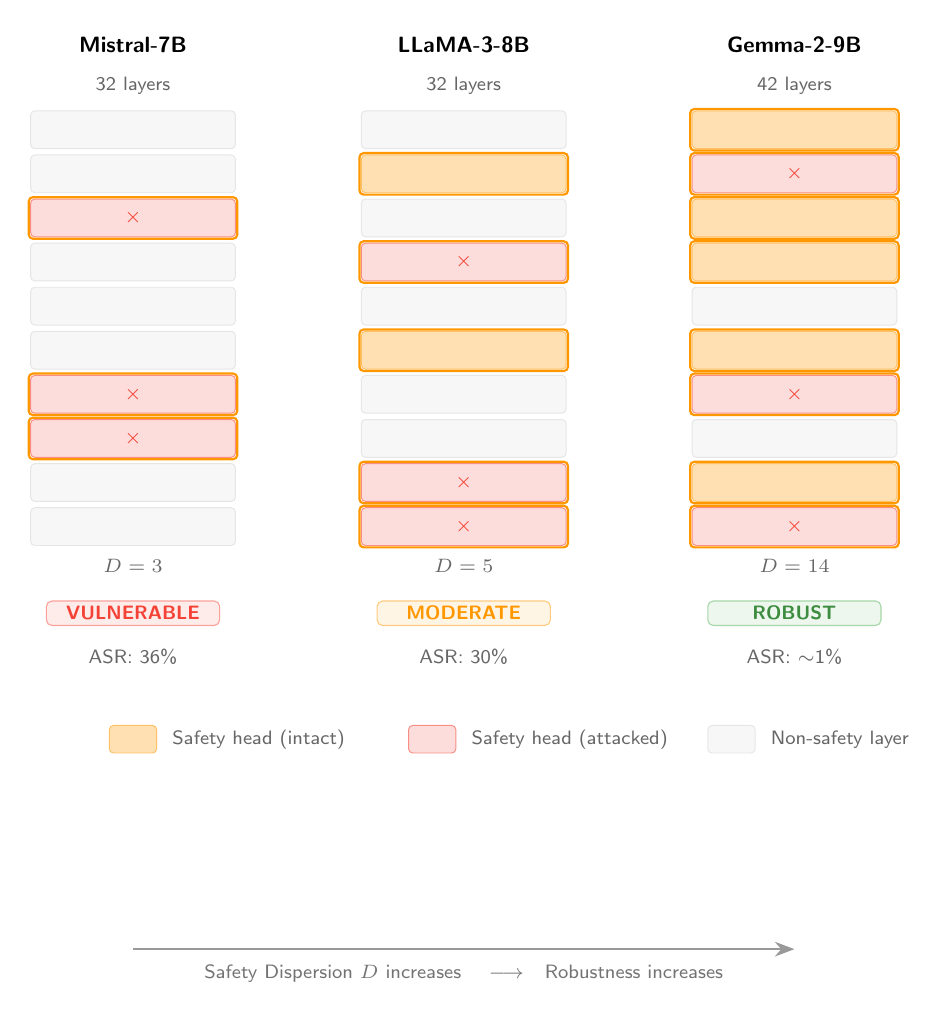
\begin{tikzpicture}[
    >=Stealth,
    font=\sffamily\small,
    layer/.style={minimum width=2.6cm, minimum height=4.8mm,
                  rounded corners=1.5pt, inner sep=0pt,
                  line width=0.35pt},
    safetylayer/.style={layer, draw=chead!60, fill=chead!30},
    offlayer/.style={layer, draw=cheadoff!80, fill=cheadoff!25},
    attacked/.style={layer, draw=cadv!60, fill=cadv!18},
    modellabel/.style={font=\sffamily\footnotesize\bfseries,
                       anchor=south},
    annot/.style={font=\sffamily\scriptsize, text=black!60},
    verdict/.style={font=\sffamily\scriptsize\bfseries, rounded corners=2pt,
                    inner xsep=4pt, inner ysep=2pt, minimum width=2.2cm},
]

% Vertical spacing
\def\vs{0.56}
\def\nlayers{10}  % abstract representation of many layers

% =====================================================================
% COLUMN 1 — Mistral (D=3)
% =====================================================================
\begin{scope}[local bounding box=col1]
  \node[modellabel] at (0, {\nlayers*\vs + 0.3}) {Mistral-7B};
  \node[annot] at (0, {\nlayers*\vs + 0.0}) {32 layers};

  % Layers (bottom=0 to top)
  \foreach \i in {0,...,9} {
    \pgfmathtruncatemacro{\layernum}{\i}
    % Safety layers: 2, 3, 7 (representing layers 2, 11, 12)
    \ifnum\i=2  \def\lstyle{attacked}\else
    \ifnum\i=3  \def\lstyle{attacked}\else
    \ifnum\i=7  \def\lstyle{attacked}\else
                \def\lstyle{offlayer}\fi\fi\fi
    \node[\lstyle] (m\i) at (0, {\i*\vs}) {};
  }
  % Original safety markers (orange outline before attack)
  \foreach \i in {2,3,7} {
    \draw[chead, line width=0.8pt, rounded corners=1.5pt]
      ([xshift=-0.5pt, yshift=-0.5pt]m\i.south west)
      rectangle ([xshift=0.5pt, yshift=0.5pt]m\i.north east);
  }

  % X marks on attacked layers
  \foreach \i in {2,3,7} {
    \node[font=\sffamily\bfseries\scriptsize, text=cadv] at (m\i) {$\times$};
  }

  \node[annot] at (0, {-0.5}) {$D = 3$};
  \node[verdict, draw=cadv!50, fill=cadv!10, text=cadv]
    at (0, {-1.1}) {VULNERABLE};
  \node[annot] at (0, {-1.65}) {ASR: 36\%};
\end{scope}

% =====================================================================
% COLUMN 2 — LLaMA-3 (D=5)
% =====================================================================
\begin{scope}[shift={(4.2, 0)}, local bounding box=col2]
  \node[modellabel] at (0, {\nlayers*\vs + 0.3}) {LLaMA-3-8B};
  \node[annot] at (0, {\nlayers*\vs + 0.0}) {32 layers};

  \foreach \i in {0,...,9} {
    % Safety layers: 0, 1, 4, 6, 8 (representing 0, 5, 9, 13, 18)
    \ifnum\i=0  \def\lstyle{attacked}\else
    \ifnum\i=1  \def\lstyle{attacked}\else
    \ifnum\i=4  \def\lstyle{safetylayer}\else  % survives
    \ifnum\i=6  \def\lstyle{attacked}\else
    \ifnum\i=8  \def\lstyle{safetylayer}\else  % survives
                \def\lstyle{offlayer}\fi\fi\fi\fi\fi
    \node[\lstyle] (l\i) at (0, {\i*\vs}) {};
  }
  \foreach \i in {0,1,4,6,8} {
    \draw[chead, line width=0.8pt, rounded corners=1.5pt]
      ([xshift=-0.5pt, yshift=-0.5pt]l\i.south west)
      rectangle ([xshift=0.5pt, yshift=0.5pt]l\i.north east);
  }

  % X marks on attacked layers
  \foreach \i in {0,1,6} {
    \node[font=\sffamily\bfseries\scriptsize, text=cadv] at (l\i) {$\times$};
  }

  \node[annot] at (0, {-0.5}) {$D = 5$};
  \node[verdict, draw=cmoderate!50, fill=cmoderate!10, text=cmoderate]
    at (0, {-1.1}) {MODERATE};
  \node[annot] at (0, {-1.65}) {ASR: 30\%};
\end{scope}

% =====================================================================
% COLUMN 3 — Gemma (D=14)
% =====================================================================
\begin{scope}[shift={(8.4, 0)}, local bounding box=col3]
  \node[modellabel] at (0, {\nlayers*\vs + 0.3}) {Gemma-2-9B};
  \node[annot] at (0, {\nlayers*\vs + 0.0}) {42 layers};

  \foreach \i in {0,...,9} {
    % Almost all are safety layers; only 2 and 5 are off
    \ifnum\i=0  \def\lstyle{attacked}\else
    \ifnum\i=1  \def\lstyle{safetylayer}\else
    \ifnum\i=2  \def\lstyle{offlayer}\else
    \ifnum\i=3  \def\lstyle{attacked}\else
    \ifnum\i=4  \def\lstyle{safetylayer}\else
    \ifnum\i=5  \def\lstyle{offlayer}\else
    \ifnum\i=6  \def\lstyle{safetylayer}\else
    \ifnum\i=7  \def\lstyle{safetylayer}\else
    \ifnum\i=8  \def\lstyle{attacked}\else
    \ifnum\i=9  \def\lstyle{safetylayer}\fi\fi\fi\fi\fi\fi\fi\fi\fi\fi
    \node[\lstyle] (g\i) at (0, {\i*\vs}) {};
  }
  \foreach \i in {0,1,3,4,6,7,8,9} {
    \draw[chead, line width=0.8pt, rounded corners=1.5pt]
      ([xshift=-0.5pt, yshift=-0.5pt]g\i.south west)
      rectangle ([xshift=0.5pt, yshift=0.5pt]g\i.north east);
  }

  % X marks on attacked layers
  \foreach \i in {0,3,8} {
    \node[font=\sffamily\bfseries\scriptsize, text=cadv] at (g\i) {$\times$};
  }

  \node[annot] at (0, {-0.5}) {$D = 14$};
  \node[verdict, draw=ccomply!50, fill=ccomply!10, text=ccomply!80!black]
    at (0, {-1.1}) {ROBUST};
  \node[annot] at (0, {-1.65}) {ASR: ${\sim}$1\%};
\end{scope}

% =====================================================================
% Legend
% =====================================================================
\begin{scope}[shift={(0, -2.7)}]
  \node[safetylayer, minimum width=6mm, minimum height=3.5mm] (legOK) at (0,0) {};
  \node[right=2pt of legOK, annot] {Safety head (intact)};

  \node[attacked, minimum width=6mm, minimum height=3.5mm] (legATK) at (3.8,0) {};
  \node[right=2pt of legATK, annot] {Safety head (attacked)};

  \node[offlayer, minimum width=6mm, minimum height=3.5mm] (legOFF) at (7.6,0) {};
  \node[right=2pt of legOFF, annot] {Non-safety layer};
\end{scope}

% =====================================================================
% Bottom arrow
% =====================================================================
\draw[->, line width=0.9pt, black!40]
  ([yshift=-3.5cm]col1.south) -- ([yshift=-3.5cm]col3.south)
  node[midway, below=2pt, font=\sffamily\scriptsize, text=black!55]
  {Safety Dispersion $D$ increases \quad$\longrightarrow$\quad Robustness increases};

\end{tikzpicture}
\end{document}
